\documentclass[aspectratio=169,12pt]{beamer}
% Visual style preserved from the supplied lecture0 template.
\usepackage[T1]{fontenc}
\usepackage[utf8]{inputenc}
\usepackage{lmodern}
\usepackage{amsmath,amssymb,mathtools}
\usepackage{tikz}
\usetikzlibrary{arrows.meta,positioning,shapes.geometric}
\usepackage{array}
\usepackage{hyperref}
\usepackage{graphicx}


\definecolor{slideorange}{HTML}{FF5500}
\definecolor{bulletgreen}{HTML}{A8C9A0}
\definecolor{bulletgray}{HTML}{D9E1E8}
\definecolor{warningred}{HTML}{F12A16}
\definecolor{rulegray}{HTML}{C9CED3}

\hypersetup{
  colorlinks=true,
  urlcolor=black,
  linkcolor=black
}
\urlstyle{same}

\setbeamertemplate{navigation symbols}{}
\setbeamercolor{background canvas}{bg=white}
\setbeamercolor{normal text}{fg=black,bg=white}
\setbeamercolor{frametitle}{fg=slideorange,bg=white}
\setbeamercolor{page number in head/foot}{fg=black,bg=white}
\setbeamerfont{frametitle}{series=\bfseries,size=\LARGE}
\setbeamerfont{page number in head/foot}{size=\scriptsize}
\setbeamersize{text margin left=0.85cm,text margin right=0.85cm}

\setbeamertemplate{frametitle}{%
  \vspace*{0.18cm}%
  \begin{beamercolorbox}[wd=\paperwidth,center,sep=0.08cm]{frametitle}
    \usebeamerfont{frametitle}\insertframetitle
  \end{beamercolorbox}%
  \vspace*{0.12cm}%
}

\setbeamertemplate{footline}{%
  \leavevmode
  \begin{beamercolorbox}[wd=\paperwidth,ht=0.42cm,dp=0.15cm,center]{page number in head/foot}
    \insertframenumber
  \end{beamercolorbox}%
}

\setbeamertemplate{itemize item}{%
  \raisebox{0.15ex}{\tikz\fill[bulletgreen] (0,0) circle (0.082cm);}%
}
\setbeamertemplate{itemize subitem}{%
  \raisebox{0.15ex}{\tikz\fill[bulletgray] (0,0) circle (0.064cm);}%
}

\newcommand{\SectionSlide}[1]{%
  \begin{frame}
    \centering
    \vfill
    {\color{slideorange}\Large\bfseries #1\par}
    \vfill
  \end{frame}
}

\newcommand{\SourceNote}[1]{%
  \vfill
  \begin{flushright}
    {\scriptsize #1}
  \end{flushright}
}


\usepackage{booktabs}
\usepackage{pgfplots}
\pgfplotsset{compat=1.18}
\usetikzlibrary{matrix,fit,calc,backgrounds}
\definecolor{forestgreen}{HTML}{4C7954}
\setbeamercolor{enumerate item}{fg=forestgreen}
\setbeamercolor{enumerate subitem}{fg=forestgreen}
\setbeamercolor{block title}{fg=slideorange,bg=white}
\setbeamercolor{block body}{fg=black,bg=white}
\newcommand{\E}{\mathbb E}
\newcommand{\Var}{\operatorname{Var}}
\newcommand{\Gain}{\operatorname{Gain}}
\newcommand{\sigmoid}{\operatorname{sigmoid}}
\newcommand{\src}[1]{\SourceNote{#1}}
\newcommand{\spaceditems}{\setlength{\itemsep}{0.30cm}}
\tikzset{
  decision/.style={draw=black,rounded corners=3pt,fill=bulletgray!25,align=center,minimum height=.70cm,inner sep=7pt,font=\small},
  leaf/.style={draw=forestgreen,rounded corners=3pt,fill=bulletgreen!20,align=center,minimum height=.65cm,inner sep=7pt,font=\small},
  orangebox/.style={draw=slideorange,rounded corners=3pt,fill=slideorange!5,align=center,minimum height=.7cm,inner sep=7pt,font=\small},
  flow/.style={-{Latex[length=2.5mm]},line width=.8pt},
  treeline/.style={line width=.8pt},
}
\hypersetup{pdftitle={Decision Trees, Random Forests, and XGBoost},pdfauthor={Zihan Zhang},pdfsubject={COMP 5212 Machine Learning}}
\pdfstringdefDisableCommands{\def\translate#1{#1}}

\newcommand{\SectionSlideN}[2]{%
	\begin{frame}
		\centering
		\vfill
		{\color{slideorange}\fontsize{29}{34}\selectfont\bfseries #1\par}
		\vspace{0.38cm}
		{\color{midgray}\fontsize{16}{21}\selectfont #2\par}
		\vfill
	\end{frame}
}
\definecolor{slideorange}{HTML}{FF5500}
\definecolor{midgray}{HTML}{666666}

\begin{document}

% 1 ---------------------------------------------------------------------------
\begin{frame}
	\begin{tikzpicture}[remember picture, overlay]
		\node[anchor=north west, inner sep=10pt] at (current page.north west)
		{
\includegraphics[width=6cm]{../source/logo.png}};
	\end{tikzpicture}
	
	\centering
	\vspace*{1.15cm}
	{\fontsize{28}{32}\selectfont COMP 5212\par}
	\vspace{0.35cm}
	{\fontsize{30}{33}\selectfont Machine Learning\par}
	\vspace{0.75cm}
	{\Large Instructor: Zihan Zhang\par}
	\vspace{0.35cm}
	{\large Lecture 7: Decision Tree, Random Forest and XGboost\par}
	
\end{frame}
% 2 ---------------------------------------------------------------------------
\begin{frame}{Learning Goals}
	  %	\centering
  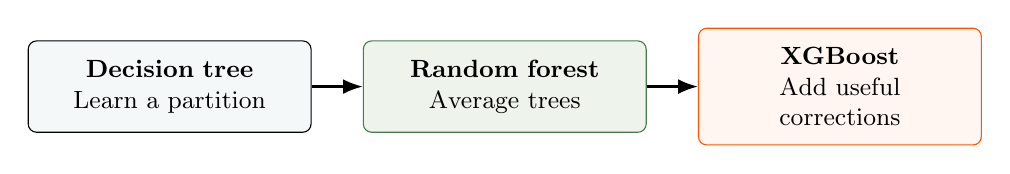
\begin{tikzpicture}[node distance=.65cm]
    \node[decision,text width=3.1cm] (dt) {\textbf{Decision tree}\\Learn a partition};
    \node[leaf,text width=3.1cm,right=of dt] (rf) {\textbf{Random forest}\\Average trees};
    \node[orangebox,text width=3.1cm,right=of rf] (xgb) {\textbf{XGBoost}\\Add useful corrections};
    \draw[flow] (dt)--(rf); \draw[flow] (rf)--(xgb);
  \end{tikzpicture}
  \vspace{.5cm}
  
\noindent By the end of the lecture, you should be able to:
	\begin{itemize}\setlength{\itemsep}{.24cm}
		\item explain the high-level idea of ensemble learning
		\item explain how AdaBoost combines simple rules into a stronger classifier;
		\item connect residual fitting to gradient descent in prediction space;
	\end{itemize}

\end{frame}

	\SectionSlideN{Decision Trees}{}
% 3 ---------------------------------------------------------------------------
\begin{frame}{A Tree Partitions the Feature Space}
	\begin{columns}[c,onlytextwidth]
		\column{.47\textwidth}
		\centering
		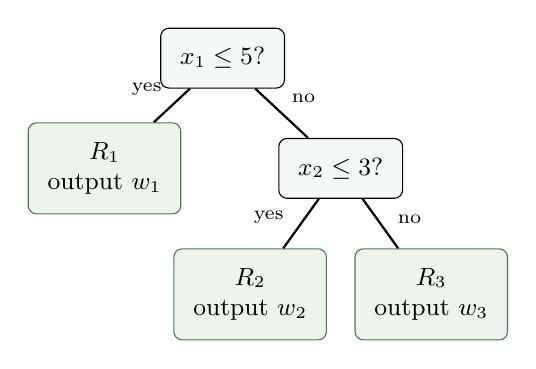
\begin{tikzpicture}
			\node[decision] (r) at (0,0) {$x_1\le 5$?};
			\node[leaf] (a) at (-1.5,-1.4) {$R_1$\\output $w_1$};
			\node[decision] (b) at (1.5,-1.4) {$x_2\le 3$?};
			\node[leaf] (c) at (.35,-3) {$R_2$\\output $w_2$};
			\node[leaf] (d) at (2.65,-3) {$R_3$\\output $w_3$};
			\draw[treeline] (r)--node[above left,font=\scriptsize]{yes}(a);
			\draw[treeline] (r)--node[above right,font=\scriptsize]{no}(b);
			\draw[treeline] (b)--node[pos=.7,above left,font=\scriptsize]{yes}(c);
			\draw[treeline] (b)--node[pos=.7,above right,font=\scriptsize]{no}(d);
		\end{tikzpicture}
		\column{.47\textwidth}
		\centering
		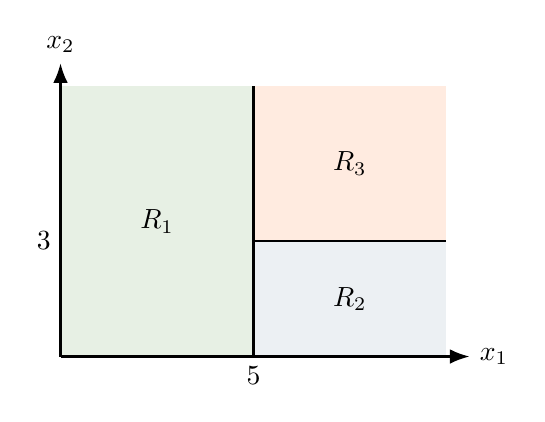
\begin{tikzpicture}[x=.49cm,y=.49cm]
			\fill[bulletgreen!28] (0,0) rectangle (5,7);
			\fill[bulletgray!50] (5,0) rectangle (10,3);
			\fill[slideorange!12] (5,3) rectangle (10,7);
			\draw[flow] (0,0)--(10.6,0) node[right]{$x_1$};
			\draw[flow] (0,0)--(0,7.6) node[above]{$x_2$};
			\draw[thick] (5,0)--(5,7); \draw[thick] (5,3)--(10,3);
			\node at (2.5,3.5) {$R_1$}; \node at (7.5,1.5) {$R_2$}; \node at (7.5,5) {$R_3$};
			\node[below] at (5,0) {5}; \node[left] at (0,3) {3};
		\end{tikzpicture}
	\end{columns}
	\pause
	\vspace{.3cm}
	\[f(x)=\sum_{v=1}^{J}w_v\,\mathbf 1\{x\in R_v\}.\]
	\centering Each leaf defines a region with a constant prediction.
\end{frame}

% 4 ---------------------------------------------------------------------------
\begin{frame}{What Does a Leaf Predict?}
	\begin{columns}[T,onlytextwidth]
		\column{.47\textwidth}
		{\large\color{slideorange}\textbf{Regression}}
		\vspace{.25cm}
		\par For squared error, use the mean target in the leaf:
		\[w_v=\frac{1}{|I_v|}\sum_{i\in I_v}y_i.\]
		\vspace{.15cm}
		\centering
		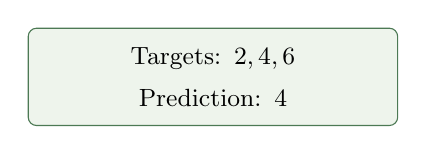
\begin{tikzpicture}
			\node[leaf,text width=4.2cm] {Targets: $2,4,6$\\[4pt]Prediction: $4$};
		\end{tikzpicture}
		\column{.47\textwidth}
		{\large\color{slideorange}\textbf{Classification}}
		\vspace{.25cm}
		\par Estimate class proportions in the leaf:
		\[p_v(c)=\frac{\sum_{i\in I_v}\mathbf 1\{y_i=c\}}{|I_v|}.\]
		\vspace{.15cm}
		\centering
		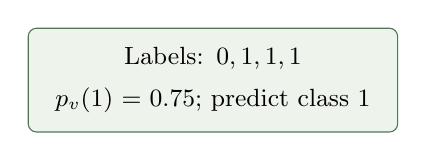
\begin{tikzpicture}
			\node[leaf,text width=4.2cm] {Labels: $0,1,1,1$\\[4pt]$p_v(1)=0.75$; predict class $1$};
		\end{tikzpicture}
	\end{columns}
	\vspace{.6cm}
	$I_v$: training samples reaching leaf $v$; $J$: number of leaves.
\end{frame}

% 5 ---------------------------------------------------------------------------
\begin{frame}{Choose a Criterion, Then Compare Splits}
	Split the samples $I$ into children $I_L$ and $I_R$.\par
	Let $A(I)$ be node impurity or average prediction loss.
	\[
	\Delta=A(I)-\frac{|I_L|}{|I|}A(I_L)-\frac{|I_R|}{|I|}A(I_R).
	\]
	\centering Select the allowed split with the largest decrease.
	\pause
	\vspace{.45cm}
	\begin{columns}[T,onlytextwidth]
		\column{.47\textwidth}
		{\large\color{slideorange}\textbf{Regression}}\par
		\vspace{.2cm}
		Squared error: use a leaf mean.\par
		\vspace{.2cm}
		Absolute error: use a leaf median.
		\column{.47\textwidth}
		{\large\color{slideorange}\textbf{Classification}}\par
		\vspace{.2cm}
		Gini impurity or entropy.\par
		\vspace{.2cm}
		Prefer purer child nodes.
	\end{columns}
	\src{Weight each child by its fraction of the samples. The criterion is a modeling choice.}
\end{frame}

% 6 ---------------------------------------------------------------------------
\begin{frame}{Regression: Minimize Squared Error}
	\setlength{\abovedisplayskip}{5pt}\setlength{\belowdisplayskip}{5pt}
	\setlength{\abovedisplayshortskip}{3pt}\setlength{\belowdisplayshortskip}{5pt}
	\textbf{SSE: sum of squared errors.} For a leaf containing samples $I$,
	\[\mathrm{SSE}(I)=\sum_{i\in I}(y_i-\bar y_I)^2,
	\qquad \mathrm{MSE}(I)=\frac{\mathrm{SSE}(I)}{|I|}.\]
	\centering
	\renewcommand{\arraystretch}{1.1}
	\begin{tabular}{c|rrrr}
		Feature $x$ & 1 & 2 & 3 & 4\\
		Target $y$ & 1 & 2 & 8 & 9
	\end{tabular}
	\vspace{.5cm}
	\begin{columns}[T,onlytextwidth]
		\column{.46\textwidth}
		\textbf{One leaf}
		\[\bar y=5,\qquad \mathrm{SSE}=50.\]
		\column{.49\textwidth}
		\pause
		\textbf{Split at $x\le2.5$}
		\[w_L=1.5,\qquad w_R=8.5,\]
		\[\mathrm{SSE}_L+\mathrm{SSE}_R=1.\]
	\end{columns}
	\pause
	\vspace{.05cm}
	\[\Delta_{\mathrm{MSE}}=
	\frac{\mathrm{SSE}(I)-\mathrm{SSE}(I_L)-\mathrm{SSE}(I_R)}{|I|}.\]
\end{frame}

% 7 ---------------------------------------------------------------------------
\begin{frame}{Classification: Gini or Entropy}
	\setlength{\abovedisplayskip}{5pt}\setlength{\belowdisplayskip}{5pt}
	\setlength{\abovedisplayshortskip}{3pt}\setlength{\belowdisplayshortskip}{5pt}
	Let $p_c$ be the fraction of samples in class $c$ at the node.
	\vspace{.3cm}
	\begin{columns}[T,onlytextwidth]
		\column{.47\textwidth}
		{\large\color{slideorange}\textbf{Gini impurity}}\par
		\[G(I)=1-\sum_{c=1}^{C}p_c^2.\]
		Measures class mixing.
		\column{.47\textwidth}
		\pause
		{\large\color{slideorange}\textbf{Entropy}}\par
		\[H(I)=-\sum_{c=1}^{C}p_c\log_2 p_c.\]
		Label uncertainty in bits; $0\log_2 0=0$.
	\end{columns}
	\pause
	\vspace{.2cm}
	\centering
	\renewcommand{\arraystretch}{1.15}
	\begin{tabular}{lcc}
		\toprule
		Binary class proportions & Gini & Entropy\\ \midrule
		Pure: $(1,0)$ & $0$ & $0$\\
		Balanced: $(0.5,0.5)$ & $0.5$ & $1$\\ \bottomrule
	\end{tabular}
	\vspace{.2cm}
	\par Both favor pure nodes, but may choose different splits.
\end{frame}

% 8 ---------------------------------------------------------------------------
\begin{frame}{One Split, Two Impurity Measures}
	\setlength{\abovedisplayskip}{5pt}\setlength{\belowdisplayskip}{5pt}
	\setlength{\abovedisplayshortskip}{3pt}\setlength{\belowdisplayshortskip}{5pt}
	\centering
	\renewcommand{\arraystretch}{1.1}
	\begin{tabular}{lcccc}
		\toprule
		Node & Class 0 & Class 1 & Gini $G$ & Entropy $H$\\ \midrule
		Parent & 4 & 4 & $0.500$ & $1.0000$\\
		Left child & 3 & 1 & $0.375$ & $0.8113$\\
		Right child & 1 & 3 & $0.375$ & $0.8113$\\ \bottomrule
	\end{tabular}
	\pause
	\vspace{.1cm}
	\par\textbf{Gini decrease}
	\[\Delta_G=0.5-\frac48(0.375)-\frac48(0.375)=0.125.\]
	\pause
	\par\textbf{Entropy decrease: information gain}
	\[\Delta_H=1-\frac48(0.8113)-\frac48(0.8113)\approx0.1887\text{ bits}.\]
	\centering Gain scales differ: compare candidates within one criterion.
\end{frame}

% 9 ---------------------------------------------------------------------------
\begin{frame}{Grow the Tree One Split at a Time}
	\begin{enumerate}\spaceditems
		\item Start with all training samples at the root.
		\item At a node, score candidate feature--threshold pairs using the chosen criterion.
		\pause
		\item Choose the best allowed split and send samples to its children.
		\item Repeat until a stopping condition is reached; assign leaf outputs.
	\end{enumerate}
	\pause
	\vspace{.35cm}
	\begin{columns}[T,onlytextwidth]
		\column{.47\textwidth}
		\textbf{Local search}\par
		An early split changes every later decision in its subtree.
		\column{.47\textwidth}
		\textbf{Computational shortcut}\par
		Sort a numerical feature and scan candidate cut points.
	\end{columns}
	\vspace{.35cm}
	\centering Greedy splitting does not guarantee the globally best tree.
\end{frame}

% 10 ---------------------------------------------------------------------------
\begin{frame}{Control How Much the Tree Can Fit}
	\begin{columns}[c,onlytextwidth]
		\column{.46\textwidth}
		\centering
		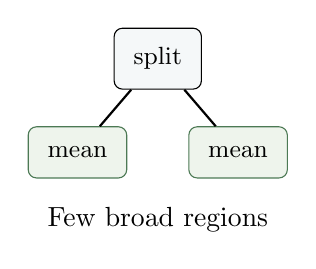
\begin{tikzpicture}[scale=.85]
			\node[decision] (r) at (0,0) {split};
			\node[leaf] (a) at (-1.2,-1.4) {mean};
			\node[leaf] (b) at (1.2,-1.4) {mean};
			\draw[treeline] (r)--(a); \draw[treeline] (r)--(b);
			\node[align=center] at (0,-2.4) {Few broad regions};
		\end{tikzpicture}
		\column{.5\textwidth}
		\begin{itemize}\spaceditems
			\item Limit maximum depth.
			\item Require enough samples in each leaf.
			\item Prune a larger tree using a complexity penalty.
		\end{itemize}
	\end{columns}
	\pause
	\vspace{.25cm}
	\[\text{Pruning objective:}\qquad R(T)+\alpha\,|\operatorname{leaves}(T)|.\]
	\centering $R(T)$: total training loss or impurity across leaves.\par
	\vspace{.2cm}
	Choose complexity on validation data; deeper trees can have higher variance.
\end{frame}

% 11 ---------------------------------------------------------------------------
\begin{frame}{Learn Where Missing Values Should Go}
	Using Gini impurity, compare both missing-value directions for $x\le5$.
	\vspace{.3cm}
	\centering
	\renewcommand{\arraystretch}{1.15}
	\begin{tabular}{c|rrrrrr}
		$x$ & 1 & 2 & 8 & 9 & missing & missing\\
		$y$ & 0 & 0 & 1 & 1 & 1 & 1
	\end{tabular}
	\pause
	\vspace{.35cm}
	\begin{tabular}{lccc}
		\toprule
		Missing direction & Left labels & Right labels & Weighted Gini\\ \midrule
		Left & $0,0,1,1$ & $1,1$ & $1/3$\\
		\textcolor{forestgreen}{Right} & $0,0$ & $1,1,1,1$ & \textcolor{forestgreen}{$0$}\\ \bottomrule
	\end{tabular}
	\pause
	\vspace{.35cm}
	\par Learn $(\text{feature},\text{threshold},\text{missing direction})$ at each node.\par
	\vspace{.2cm}
	This is a routing rule. Later splits can still separate missing samples.
\end{frame}

% 12 ---------------------------------------------------------------------------
\begin{frame}{A Surrogate Split Uses Another Feature}
	\begin{columns}[c,onlytextwidth]
		\column{.48\textwidth}
		\centering
		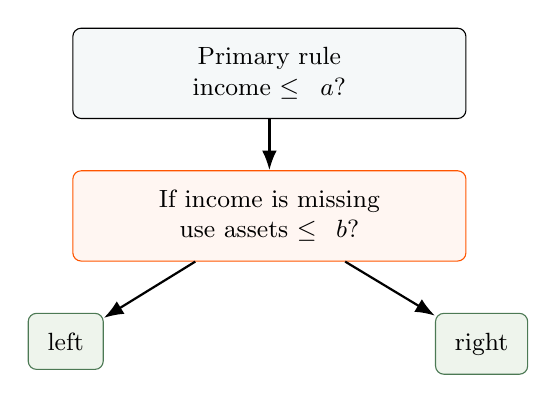
\begin{tikzpicture}[node distance=.65cm]
			\node[decision,text width=4.5cm] (a) {Primary rule\\income $\le a$?};
			\node[orangebox,text width=4.5cm,below=of a] (b) {If income is missing\\use assets $\le b$?};
			\node[leaf,below left=.65cm and -.4cm of b] (l) {left};
			\node[leaf,below right=.65cm and -.4cm of b] (r) {right};
			\draw[flow] (a)--(b); \draw[flow] (b)--(l); \draw[flow] (b)--(r);
		\end{tikzpicture}
		\column{.48\textwidth}
		\pause
		\begin{itemize}\spaceditems
			\item Find a rule that reproduces the primary split's left/right assignments.
			\item Samples missing the primary feature may take different branches.
			\item A learned default direction can also separate samples later, using other features.
		\end{itemize}
	\end{columns}
	\src{CART-style surrogate splits; illustrative rules.}
\end{frame}

% 13 ---------------------------------------------------------------------------
\begin{frame}{A Small Data Change Can Change the Tree}
	\centering
	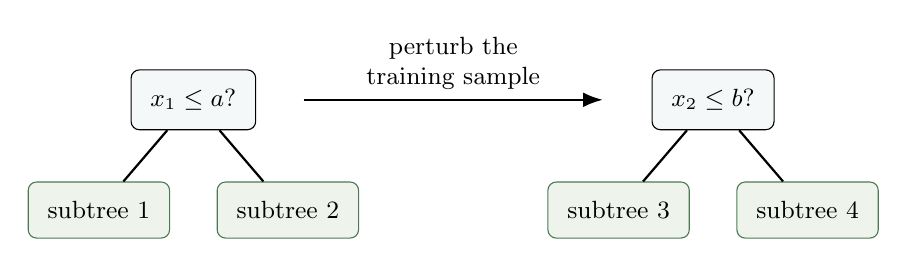
\begin{tikzpicture}
		\node[decision] (a) at (-3.3,0) {$x_1\le a$?};
		\node[leaf] (al) at (-4.5,-1.4) {subtree 1};
		\node[leaf] (ar) at (-2.1,-1.4) {subtree 2};
		\node[decision] (b) at (3.3,0) {$x_2\le b$?};
		\node[leaf] (bl) at (2.1,-1.4) {subtree 3};
		\node[leaf] (br) at (4.5,-1.4) {subtree 4};
		\draw[treeline] (a)--(al); \draw[treeline] (a)--(ar);
		\draw[treeline] (b)--(bl); \draw[treeline] (b)--(br);
		\draw[flow] (-1.9,0)--node[above,font=\small,align=center]{perturb the\\training sample}(1.9,0);
	\end{tikzpicture}
	\pause
	\vspace{.55cm}
	\begin{itemize}\spaceditems
		\item Competing splits may have very similar training scores.
		\item A different early split changes the downstream partition.
		\item Averaging many diverse trees can stabilize predictions.
	\end{itemize}
	\src{Schematic illustration of tree instability. Next: random forests.}
\end{frame}

	\SectionSlideN{Random Forests}{}
% 12 --------------------------------------------------------------------------
\begin{frame}{Random Forest: Two Sources of Randomness}
  \centering
  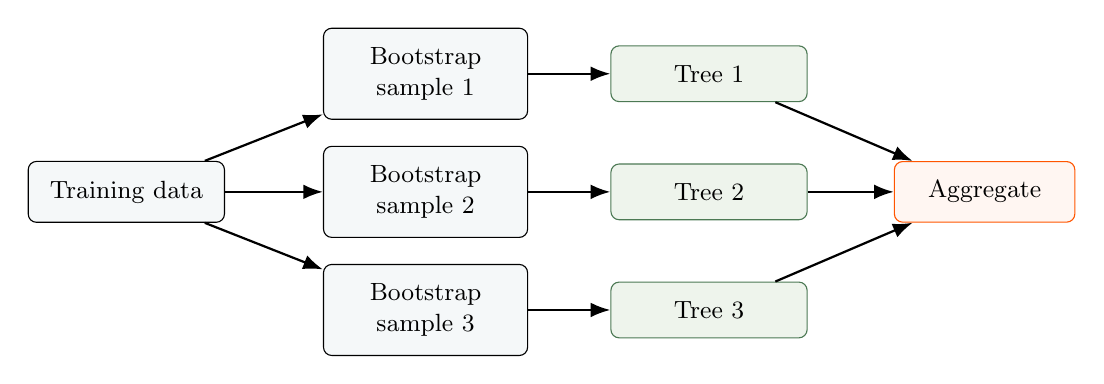
\begin{tikzpicture}
    \node[decision,text width=2cm] (data) at (0,0) {Training data};
    \foreach \k/\yy in {1/1.5,2/0,3/-1.5}{
      \node[decision,text width=2.1cm] (s\k) at (3.8,\yy) {Bootstrap sample $\k$};
      \node[leaf,text width=2cm] (t\k) at (7.4,\yy) {Tree $\k$};
      \draw[flow] (data)--(s\k); \draw[flow] (s\k)--(t\k);
    }
    \node[orangebox,text width=1.8cm] (out) at (10.9,0) {Aggregate};
    \foreach \k in {1,2,3}{\draw[flow] (t\k)--(out);}
  \end{tikzpicture}
  \vspace{.3cm}
  \begin{itemize}\spaceditems
    \item Sample training rows with replacement for each tree.
    \pause
    \item At each node, search a random subset of the features.
  \end{itemize}
  \src{Regression: average predictions. Classification: vote or average class probabilities, depending on implementation.}
\end{frame}

% 13 --------------------------------------------------------------------------
\begin{frame}{Random Features Reduce Shared Errors}
  Suppose one feature dominates the split score in many bootstrap samples.
  \vspace{.3cm}
  \begin{columns}[T,onlytextwidth]
    \column{.47\textwidth}
    \textbf{Search every feature}\par\vspace{.2cm}
    Many trees select similar early splits.\par\vspace{.2cm}
    Their prediction errors can be strongly correlated.
    \column{.47\textwidth}
    \pause
    \textbf{Search a random subset}\par\vspace{.2cm}
    Some nodes must use alternative predictors.\par\vspace{.2cm}
    Trees can become more diverse.
  \end{columns}
  \pause
  \vspace{.25cm}
  \centering
  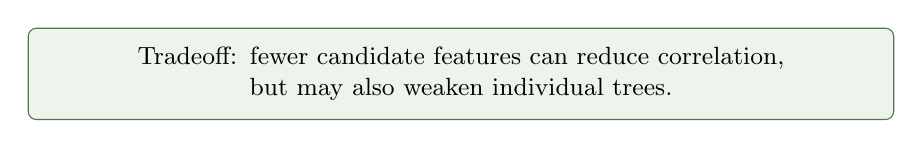
\begin{tikzpicture}
    \node[leaf,text width=10.5cm] {Tradeoff: fewer candidate features can reduce correlation,\\but may also weaken individual trees.};
  \end{tikzpicture}
\end{frame}

% 14 --------------------------------------------------------------------------
\begin{frame}{Correlation Limits the Gain from Averaging}
  At a fixed input, suppose trees have variance $\sigma^2$ and pairwise correlation $\rho$.
  \pause
  \[\Var\!\left(\frac1B\sum_{b=1}^{B}T_b(x)\right)
      =\rho\sigma^2+\frac{1-\rho}{B}\sigma^2.\]
  \pause
  \begin{columns}[c,onlytextwidth]
    \column{.56\textwidth}
    \centering
    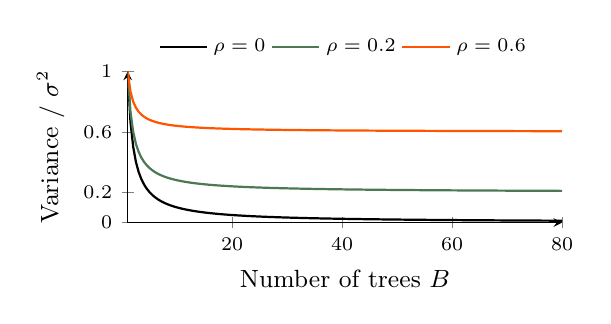
\begin{tikzpicture}
      \begin{axis}[width=7.1cm,height=3.5cm,xmin=1,xmax=80,ymin=0,ymax=1,
        xlabel={Number of trees $B$},ylabel={Variance / $\sigma^2$},
        tick label style={font=\scriptsize},label style={font=\small},
        legend style={font=\scriptsize,draw=none,at={(.5,1.03)},anchor=south,legend columns=3},
        axis lines=left,ytick={0,.2,.6,1}]
        \addplot[black,thick,domain=1:80,samples=160]{1/x};\addlegendentry{$\rho=0$}
        \addplot[forestgreen,thick,domain=1:80,samples=160]{.2+.8/x};\addlegendentry{$\rho=0.2$}
        \addplot[slideorange,thick,domain=1:80,samples=160]{.6+.4/x};\addlegendentry{$\rho=0.6$}
      \end{axis}
    \end{tikzpicture}
    \column{.4\textwidth}
    More trees reduce the second term.\par\vspace{.35cm}
    Lower correlation reduces the limiting variance.
  \end{columns}
\end{frame}

% 15 --------------------------------------------------------------------------
\begin{frame}{OOB Is Defined Separately for Each Tree}
  \centering
  \renewcommand{\arraystretch}{1.15}
  \begin{tabular}{lcccc}
    \toprule
     & Tree 1 & Tree 2 & Tree 3 & Tree 4\\ \midrule
    Sample A & in-bag & \textcolor{forestgreen}{OOB} & in-bag & \textcolor{forestgreen}{OOB}\\
    Sample B & \textcolor{forestgreen}{OOB} & in-bag & in-bag & in-bag\\
    Sample C & in-bag & in-bag & \textcolor{forestgreen}{OOB} & \textcolor{forestgreen}{OOB}\\ \bottomrule
  \end{tabular}
  \pause
  \vspace{.25cm}
  \par For sample A, aggregate predictions from trees 2 and 4 only.
  \pause
  \vspace{.35cm}
  \[\widehat f_{\mathrm{OOB}}(x_i)
    =\frac{1}{|\mathcal B_i|}\sum_{b\in\mathcal B_i}T_b(x_i),
    \qquad\mathcal B_i=\{b:i\notin D_b\},\quad |\mathcal B_i|>0.\]
  \centering Compare each sample's OOB prediction with its observed target.
  \src{Formula shown for regression; classification can aggregate OOB class probabilities.}
\end{frame}

% 16 --------------------------------------------------------------------------
\begin{frame}{OOB Depends on Draws per Tree}
  Original data: $n$ samples. Each tree draws $m$ times with replacement.
  \pause
  \[q=P(i\text{ is OOB for one tree})=
    \left(1-\frac1n\right)^m\approx e^{-m/n}.\]
  \pause
  \centering
  \renewcommand{\arraystretch}{1.15}
  \begin{tabular}{lcc}
    \toprule
    Draws per tree & OOB probability $q$ & Expected OOB trees, $B=100$\\ \midrule
    $m=n$ & $36.8\%$ & $36.8$\\
    $m=2n$ & $13.5\%$ & $13.5$\\
    $m=5n$ & $0.67\%$ & $0.67$\\ \bottomrule
  \end{tabular}
  \vspace{.3cm}
  \par Increasing $B$ gives more OOB predictions per sample.\par
  \vspace{.18cm}
  Increasing $m/n$ makes exclusion from any one tree less likely.
  \src{Large-$n$ approximations. Standard bootstrap usually takes $m=n$; $m>n$ rows are illustrative variants.}
\end{frame}

% 17 --------------------------------------------------------------------------
\begin{frame}{Random Forest for Port Energy Forecasting}
  \textbf{Valletta Cruise Port, Malta: a 2025 study}
  \vspace{.3cm}
  \begin{itemize}\spaceditems
    \item Predict next-day hourly demand to support energy scheduling.
    \item Inputs: past demand, calendar, temperature, PV generation, ship activity.
    \item 8,760 hourly records; metered baseline plus estimated shore-power demand.
  \end{itemize}
  \vspace{.4cm}
  \centering
  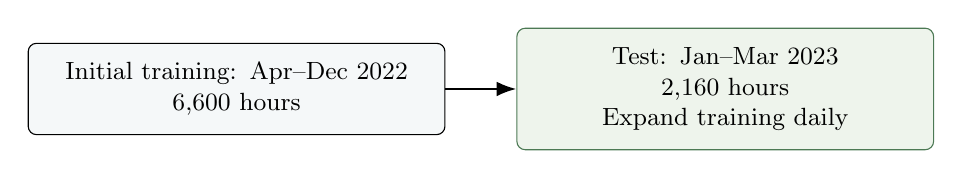
\begin{tikzpicture}[node distance=.9cm]
    \node[decision,text width=4.8cm] (tr) {Initial training: Apr--Dec 2022\\6,600 hours};
    \node[leaf,text width=4.8cm,right=of tr] (te) {Test: Jan--Mar 2023\\2,160 hours\\Expand training daily};
    \draw[flow] (tr)--(te);
  \end{tikzpicture}
\end{frame}

% 18 --------------------------------------------------------------------------
\begin{frame}{Lower Forecast Error Than Linear Regression}
  \begin{columns}[c,onlytextwidth]
    \column{.59\textwidth}
    \centering
    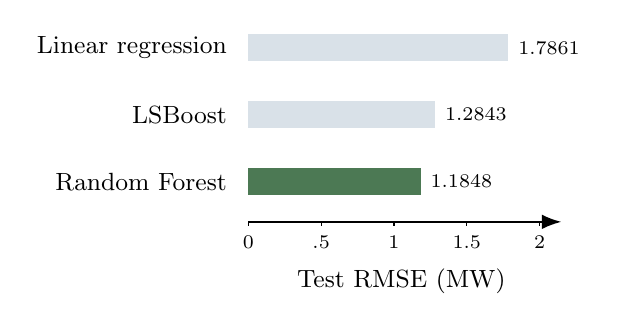
\begin{tikzpicture}[x=1.85cm,y=.85cm]
      \foreach \yy/\vv/\lab in {3/1.7861/{Linear regression},2/1.2843/{LSBoost}}{
        \fill[bulletgray] (0,\yy-.2) rectangle (\vv,\yy+.2);
        \node[anchor=east,font=\small] at (-.08,\yy) {\lab};
        \node[anchor=west,font=\scriptsize] at (\vv,\yy) {\vv};
      }
      \fill[forestgreen] (0,.8) rectangle (1.1848,1.2);
      \node[anchor=east,font=\small] at (-.08,1) {Random Forest};
      \node[anchor=west,font=\scriptsize] at (1.1848,1) {1.1848};
      \draw[flow] (0,.4)--(2.15,.4);
      \foreach \xx in {0,.5,1,1.5,2}{
        \draw (\xx,.4)--(\xx,.34);
        \node[below,font=\scriptsize] at (\xx,.34) {\xx};
      }
      \node[below,font=\small] at (1.05,-.15) {Test RMSE (MW)};
    \end{tikzpicture}
    \column{.36\textwidth}
    {\color{forestgreen}\fontsize{28}{32}\selectfont\textbf{33.7\%}}\par
    lower RMSE than linear regression.\par
    \vspace{.3cm}
    All shown models use expanding-window evaluation.
  \end{columns}
\end{frame}

	\SectionSlideN{XGboost}{}
% 19 --------------------------------------------------------------------------
\begin{frame}{Boosting Learns Successive Corrections}
  \begin{columns}[T,onlytextwidth]
    \column{.45\textwidth}
    {\large\color{slideorange}\textbf{Random forest}}
    \vspace{.25cm}
    \par Trees can be trained independently.\par
    \vspace{.25cm}
    \[\widehat f(x)=\frac1B\sum_{b=1}^{B}T_b(x).\]
    Average diverse predictions.
    \column{.51\textwidth}
    {\large\color{slideorange}\textbf{Gradient boosting}}
    \vspace{.25cm}
    \par Each new tree depends on the current model.\par
    \vspace{.25cm}
    \[F_t(x)=F_{t-1}(x)+\eta f_t(x).\]
    Add a correction to the current score.
  \end{columns}
  \vspace{.6cm}
  \centering
  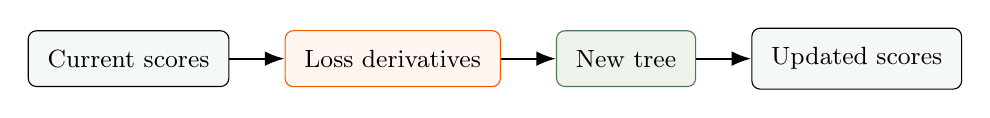
\begin{tikzpicture}[node distance=.7cm]
    \node[decision] (a) {Current scores};
    \node[orangebox,right=of a] (b) {Loss derivatives};
    \node[leaf,right=of b] (c) {New tree};
    \node[decision,right=of c] (d) {Updated scores};
    \draw[flow] (a)--(b);\draw[flow] (b)--(c);\draw[flow] (c)--(d);
  \end{tikzpicture}
  \src{Connection to AdaBoost: sequential learning; the loss determines how later learners respond to errors.}
\end{frame}

% 20 --------------------------------------------------------------------------
\begin{frame}{Squared Loss Leads to Residual Fitting}
  Start with $F_0(x)=5$. Fit a regression stump to $r_i=y_i-F_0(x_i)$.
  \vspace{.3cm}
  \centering
  \renewcommand{\arraystretch}{1.3}
  \begin{tabular}{c|rrrr}
    $x_i$ & 1 & 2 & 3 & 4\\
    $y_i$ & 1 & 2 & 8 & 9\\
    Residual $r_i$ & $-4$ & $-3$ & $3$ & $4$\\ \midrule
    \uncover<2->{Stump $f_1(x_i)$} & \uncover<2->{$-3.5$} & \uncover<2->{$-3.5$} & \uncover<2->{$3.5$} & \uncover<2->{$3.5$}\\
    \uncover<3->{$F_1(x_i)$, with $\eta=0.5$} & \uncover<3->{$3.25$} & \uncover<3->{$3.25$} & \uncover<3->{$6.75$} & \uncover<3->{$6.75$}
  \end{tabular}
  \uncover<3->{
  \vspace{.25cm}
  \[F_1(x)=5+0.5f_1(x).\]
  \centering The next tree fits what remains after this update.
  }
\end{frame}

% 21 --------------------------------------------------------------------------
\begin{frame}{A Tree Outputs a Score, Also for Classification}
  \[s(x)=b+\sum_{t=1}^{T}\eta f_t(x),\qquad f_t(x)=w_{t,q_t(x)}.\]
  \vspace{.2cm}
  \begin{columns}[T,onlytextwidth]
    \column{.47\textwidth}
    \textbf{Squared-error regression}
    \[\widehat y=s,\]
    \[\ell(y,s)=\tfrac12(s-y)^2.\]
    A leaf changes the predicted value.
    \pause
    \column{.49\textwidth}
    \textbf{Binary classification: $y\in\{0,1\}$}
    \[p=\sigma(s)=\frac{1}{1+e^{-s}},\]
    \[\ell(y,s)=\log(1+e^s)-ys.\]
    A leaf changes the logit; sigmoid gives a probability.
  \end{columns}
  \vspace{.25cm}
  \centering $q_t(x)$ identifies a leaf; $w_{t,v}$ is that leaf's real-valued output.
\end{frame}

% 22 --------------------------------------------------------------------------
\begin{frame}{One Round Optimizes One New Tree}
  Fix the existing ensemble, with current scores $s_i=F_{t-1}(x_i)$.
  \vspace{.25cm}
  \[
    \mathcal L_t(f_t)=\sum_{i=1}^{n}\ell\bigl(y_i,s_i+f_t(x_i)\bigr)
      +\Omega(f_t).
  \]
  \[
    \Omega(f_t)=\gamma J+\frac\lambda2\sum_{v=1}^{J}w_v^2.
  \]
  \pause
  \begin{itemize}\spaceditems
    \item Learn the partition and its $J$ leaf values.
    \item $\gamma$ penalizes additional leaves; $\lambda$ shrinks leaf values.
    \item First derive an unshrunk tree; apply learning rate $\eta$ afterward.
  \end{itemize}
  \src{L2-regularized scalar-tree formulation.}
\end{frame}

% 23 --------------------------------------------------------------------------
\begin{frame}{Approximate the Loss Around the Current Score}
  For each sample, expand in the proposed correction $f_t(x_i)$:
  \[
    \ell\bigl(y_i,s_i+f_t(x_i)\bigr)
    \approx \ell(y_i,s_i)+g_if_t(x_i)+\tfrac12h_if_t(x_i)^2.
  \]
  \pause
  \[g_i=\left.\frac{\partial\ell(y_i,s)}{\partial s}\right|_{s=s_i},
    \qquad h_i=\left.\frac{\partial^2\ell(y_i,s)}{\partial s^2}\right|_{s=s_i}.\]
  \pause
  \vspace{.2cm}
  Drop terms that are constant with respect to the new tree:
  \[
    \widetilde{\mathcal L}_t
     =\sum_i\left[g_if_t(x_i)+\tfrac12h_if_t(x_i)^2\right]+\Omega(f_t).
  \]
  \centering Exact for squared loss; a local approximation for logistic loss.
\end{frame}

% 24 --------------------------------------------------------------------------
\begin{frame}{The Loss Supplies Two Numbers per Sample}
  \centering
  \renewcommand{\arraystretch}{1.65}
  \begin{tabular}{lcc}
    \toprule
    Loss & Gradient $g_i$ & Hessian $h_i$\\ \midrule
    $\tfrac12(s_i-y_i)^2$ & $s_i-y_i$ & $1$\\
    Binary cross-entropy & $p_i-y_i$ & $p_i(1-p_i)$\\ \bottomrule
  \end{tabular}
  \vspace{.3cm}
  \par In classification, $p_i=\sigma(s_i)$.
  \pause
  \vspace{.5cm}
  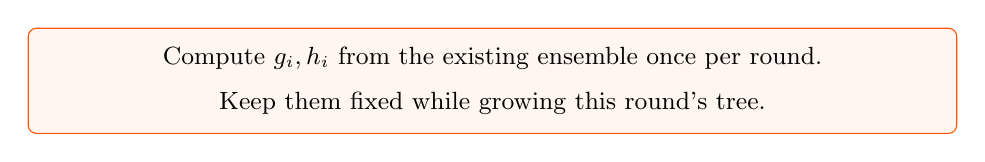
\begin{tikzpicture}
    \node[orangebox,text width=11.3cm] {Compute $g_i,h_i$ from the existing ensemble once per round.\\[5pt]
    Keep them fixed while growing this round's tree.};
  \end{tikzpicture}
  \vspace{.35cm}
  \par Candidate leaves only need sums of these statistics.
\end{frame}

% 25 --------------------------------------------------------------------------
\begin{frame}{Each Leaf Has an Optimal Constant Correction}
  For samples $I_v$ reaching leaf $v$, define
  \[G_v=\sum_{i\in I_v}g_i,\qquad H_v=\sum_{i\in I_v}h_i.\]
  \pause
  Its contribution to the approximate objective is
  \[Q_v(w_v)=G_vw_v+\frac12(H_v+\lambda)w_v^2+\gamma.\]
  \pause
  \[\frac{\partial Q_v}{\partial w_v}=G_v+(H_v+\lambda)w_v=0
    \quad\Longrightarrow\quad
    \boxed{w_v^*=-\frac{G_v}{H_v+\lambda}}.\]
  \vspace{.2cm}
  \centering For squared loss and $\lambda=0$, this is the mean residual in the leaf.
  \src{A leaf value is a score correction contributed by this tree.}
\end{frame}

% 26 --------------------------------------------------------------------------
\begin{frame}{Split Gain Chooses the Tree Structure}
  \centering
  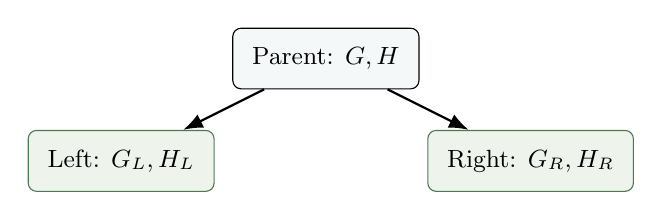
\begin{tikzpicture}
    \node[decision] (p) at (0,0) {Parent: $G,H$};
    \node[leaf] (l) at (-2.6,-1.3) {Left: $G_L,H_L$};
    \node[leaf] (r) at (2.6,-1.3) {Right: $G_R,H_R$};
    \draw[flow] (p)--(l);\draw[flow] (p)--(r);
  \end{tikzpicture}
  \pause
  \vspace{.15cm}
  \[
    \boxed{\Gain=\frac12\left[
      \frac{G_L^2}{H_L+\lambda}+\frac{G_R^2}{H_R+\lambda}
      -\frac{G^2}{H+\lambda}\right]-\gamma}
  \]
  \pause
  \begin{itemize}\setlength{\itemsep}{.2cm}
    \item Compare the optimized parent leaf with two optimized child leaves.
    \item Search candidate features and thresholds; prefer the largest allowed gain.
    \item Recurse, with growth constraints and pruning controlling complexity.
  \end{itemize}
  \src{Here $G=G_L+G_R$, $H=H_L+H_R$. The displayed gain already subtracts $\gamma$.}
\end{frame}

% 27 --------------------------------------------------------------------------
\begin{frame}{Worked Example: Start a Regularized Round}
  Restart from $s_i=5$ for all samples. Use squared loss, $\lambda=1$, $\gamma=0$.
  \vspace{.3cm}
  \centering
  \renewcommand{\arraystretch}{1.15}
  \begin{tabular}{ccccc}
    \toprule
    Feature $x_i$ & Target $y_i$ & Score $s_i$ & $g_i=s_i-y_i$ & $h_i$\\ \midrule
    1 & 1 & 5 & \uncover<2->{$4$} & \uncover<2->{1}\\
    2 & 2 & 5 & \uncover<2->{$3$} & \uncover<2->{1}\\
    3 & 8 & 5 & \uncover<2->{$-3$} & \uncover<2->{1}\\
    4 & 9 & 5 & \uncover<2->{$-4$} & \uncover<2->{1}\\ \bottomrule
  \end{tabular}
  \uncover<2->{
  \vspace{.35cm}
  \[G=0,\qquad H=4.\]
  \centering Candidate thresholds: $1.5$, $2.5$, and $3.5$.
  }
\end{frame}

% 28 --------------------------------------------------------------------------
\begin{frame}{Compare the Candidates and Set Leaf Values}
  For $x\le2.5$: $G_L=7$, $H_L=2$, $G_R=-7$, $H_R=2$.
  \[\Gain=\frac12\left[\frac{49}{3}+\frac{49}{3}-\frac0{5}\right]
      =\frac{49}{3}\approx16.33.\]
  \pause
  \begin{columns}[c,onlytextwidth]
    \column{.43\textwidth}
    \centering
    \renewcommand{\arraystretch}{1.3}
    \begin{tabular}{cc}
      \toprule
      Threshold & Gain\\ \midrule
      $1.5$ & $6$\\
      \textcolor{forestgreen}{$2.5$} & \textcolor{forestgreen}{$16.33$}\\
      $3.5$ & $6$\\ \bottomrule
    \end{tabular}
    \pause
    \column{.53\textwidth}
    \centering
    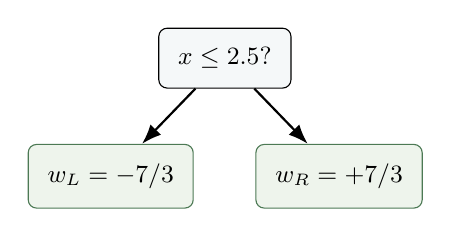
\begin{tikzpicture}
      \node[decision] (r) at (0,0) {$x\le2.5$?};
      \node[leaf] (l) at (-1.45,-1.5) {$w_L=-7/3$};
      \node[leaf] (rr) at (1.45,-1.5) {$w_R=+7/3$};
      \draw[flow] (r)--(l); \draw[flow] (r)--(rr);
    \end{tikzpicture}
  \end{columns}
  \vspace{.35cm}
  \centering The split groups samples that need similar corrections.
\end{frame}

% 29 --------------------------------------------------------------------------
\begin{frame}{Shrink the New Tree, Then Update the Scores}
  \[F_t(x)=F_{t-1}(x)+\eta f_t(x).\]
  \centering
  With $\eta=0.3$:
  \vspace{.25cm}
  \renewcommand{\arraystretch}{1.2}
  \begin{tabular}{c|rrrr}
    $x_i$ & 1 & 2 & 3 & 4\\ \midrule
    Old score & 5 & 5 & 5 & 5\\
    New tree $f_t(x_i)$ & $-7/3$ & $-7/3$ & $7/3$ & $7/3$\\
    \uncover<2->{Applied correction} & \uncover<2->{$-0.7$} & \uncover<2->{$-0.7$} & \uncover<2->{$0.7$} & \uncover<2->{$0.7$}\\
    \uncover<2->{\textbf{New score}} & \uncover<2->{\textbf{4.3}} & \uncover<2->{\textbf{4.3}} & \uncover<2->{\textbf{5.7}} & \uncover<2->{\textbf{5.7}}\\
    Target & 1 & 2 & 8 & 9
  \end{tabular}
  \vspace{.35cm}
  \par\uncover<2->{The next round recomputes gradients from these updated scores.}
\end{frame}

% 30 --------------------------------------------------------------------------
\begin{frame}{In Classification, Leaves Correct the Logit}
  A leaf contains labels $(1,1,1,0)$; currently $s_i=0$, so $p_i=0.5$.
  \pause
  \[
    G_v=(-0.5)+(-0.5)+(-0.5)+0.5=-1,\qquad H_v=4(0.25)=1.
  \]
  With $\lambda=0$, the leaf value is $w_v=-G_v/H_v=1$.
  \pause
  \vspace{.4cm}
  \centering
  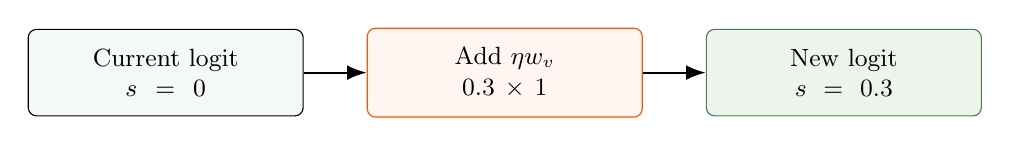
\begin{tikzpicture}[node distance=.8cm]
    \node[decision,text width=3cm] (a) {Current logit\\$s=0$};
    \node[orangebox,text width=3cm,right=of a] (b) {Add $\eta w_v$\\$0.3\times1$};
    \node[leaf,text width=3cm,right=of b] (c) {New logit\\$s=0.3$};
    \draw[flow] (a)--(b); \draw[flow] (b)--(c);
  \end{tikzpicture}
  \vspace{.3cm}
  \[p_{\mathrm{new}}=\sigma(0.3)\approx0.574.\]
  \centering Sum tree outputs first; apply sigmoid to the ensemble score.
\end{frame}

% 31 --------------------------------------------------------------------------
\begin{frame}{One XGBoost Round, End to End}
  \begin{enumerate}\setlength{\itemsep}{.32cm}
    \item Compute current ensemble scores $s_i$ and derivatives $g_i,h_i$.
    \item Start a tree at the root; aggregate $G,H$ for its samples.
    \pause
    \item Search feature--threshold candidates using split gain.
    \item Continue growing subject to constraints; set final leaf values.
    \pause
    \item Update $s_i\leftarrow s_i+\eta w_{q_t(x_i)}$.
  \end{enumerate}
  \vspace{.3cm}
  \centering
  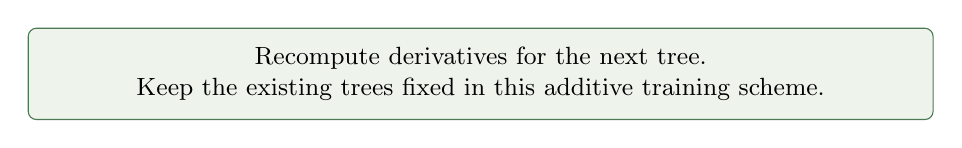
\begin{tikzpicture}
    \node[leaf,text width=11cm] {Recompute derivatives for the next tree.\\Keep the existing trees fixed in this additive training scheme.};
  \end{tikzpicture}
\end{frame}

% 32 --------------------------------------------------------------------------
\begin{frame}{Regularization Acts at Several Levels}
  \centering
  \small\renewcommand{\arraystretch}{1.15}
  \begin{tabular}{>{\raggedright\arraybackslash}p{4.1cm}>{\raggedright\arraybackslash}p{8.0cm}}
    \toprule
    Control & What it changes\\ \midrule
    Maximum depth & Limits the complexity of interactions in one tree.\\
    \texttt{min\_child\_weight} & Requires enough Hessian mass $H$ in each child.\\
    $\lambda$ and $\gamma$ & Shrink leaf values and penalize extra leaves.\\
    Learning rate $\eta$ & Shrinks each tree's contribution to the ensemble.\\
    Row/feature subsampling & Adds randomness during tree construction.\\ \bottomrule
  \end{tabular}
  \vspace{.4cm}
  \normalsize\par Select boosting rounds on validation data.\par
  Reserve the test set for final evaluation.
\end{frame}

% 33 --------------------------------------------------------------------------
\begin{frame}{XGBoost for Early Sepsis Prediction}
  \textbf{A 2023 study: predict sepsis within the next six hours.}
  \vspace{.3cm}
  \begin{itemize}\spaceditems
    \item 4,603 trauma patients in MIMIC-IV; one hospital, 2008--2019.
    \item Clinical variables, measurement patterns, and time-series features.
    \item Compare XGBoost with L2-regularized logistic regression.
  \end{itemize}
  \vspace{.25cm}
  \centering
  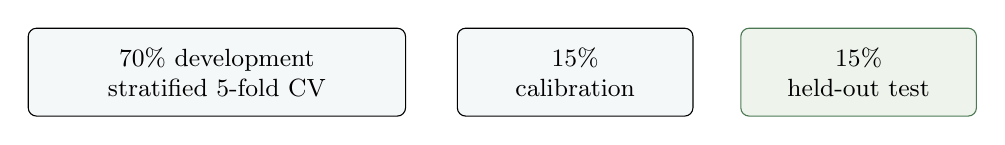
\begin{tikzpicture}
    \node[decision,text width=4.3cm] (a) at (0,0) {70\% development\\stratified 5-fold CV};
    \node[decision,text width=2.5cm] (b) at (4.55,0) {15\%\\calibration};
    \node[leaf,text width=2.5cm] (c) at (8.15,0) {15\%\\held-out test};
  \end{tikzpicture}
  \vspace{.3cm}
  \par Random patient-level split: each patient's records stay together.
\end{frame}

% 34 --------------------------------------------------------------------------
\begin{frame}{XGBoost vs. Logistic Regression}
  \centering
  Six-hour prediction window; time-step-level evaluation.
  \vspace{.25cm}
  \renewcommand{\arraystretch}{1.3}
  \begin{tabular}{lcc}
    \toprule
    Model & AUROC (95\% CI) & AUPRC (95\% CI)\\ \midrule
    L2 logistic regression & $0.83\;(0.81,0.85)$ & $0.18\;(0.15,0.21)$\\
    \textcolor{forestgreen}{XGBoost} & \textcolor{forestgreen}{$0.87\;(0.85,0.89)$} & \textcolor{forestgreen}{$0.27\;(0.23,0.31)$}\\ \bottomrule
  \end{tabular}
  \vspace{.35cm}
  \par AUROC: area under the ROC curve.\par
  AUPRC: area under the precision--recall curve. Higher is better.
  \vspace{.3cm}
  \par Retrospective test results; clinical benefit and external generalization were not established.
\end{frame}

% 35 --------------------------------------------------------------------------
\begin{frame}{XGBoost in Production: Uber, 2026}
  \textbf{Detect bounding-box annotation errors before submission.}
  \vspace{.4cm}
  \centering
  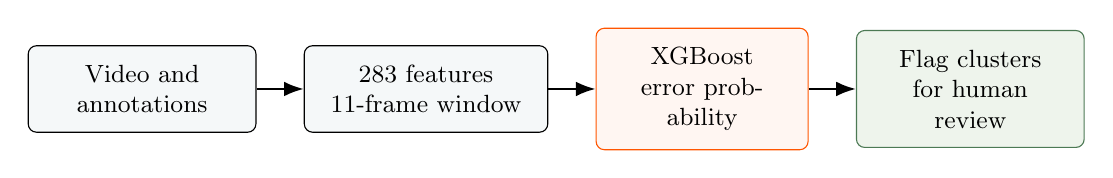
\begin{tikzpicture}[node distance=.6cm]
    \node[decision,text width=2.4cm] (a) {Video and\\annotations};
    \node[decision,text width=2.6cm,right=of a] (b) {283 features\\11-frame window};
    \node[orangebox,text width=2.2cm,right=of b] (c) {XGBoost\\error probability};
    \node[leaf,text width=2.4cm,right=of c] (d) {Flag clusters\\for human review};
    \draw[flow] (a)--(b);\draw[flow] (b)--(c);\draw[flow] (c)--(d);
  \end{tikzpicture}
  \vspace{.4cm}
  \begin{itemize}\spaceditems
    \item Visual, motion, and geometric features summarize video context.
    \item Training anomalies simulate tracking jumps and identity swaps.
    \item Deployed across Uber's bounding-box annotation projects.
  \end{itemize}
\end{frame}


\begin{frame}{Three Models, Three Training Strategies}
  \centering
  \small\renewcommand{\arraystretch}{1.15}
  \begin{tabular}{>{\raggedright\arraybackslash}p{2.1cm}>{\raggedright\arraybackslash}p{3.0cm}>{\raggedright\arraybackslash}p{3.3cm}>{\raggedright\arraybackslash}p{3.5cm}}
    \toprule
     & \textbf{Single tree} & \textbf{Random forest} & \textbf{XGBoost}\\ \midrule
    Training & Greedy splits & Bootstrap + random features & Sequential loss-based corrections\\
    Combine & One partition & Average or vote & Sum of score increments\\
    Main benefit & Simple rules & Lower variance & Flexible loss minimization\\
    Main controls & Depth, leaf size & Feature subset, leaf size, trees & Depth, regularization, learning rate, rounds\\ \bottomrule
  \end{tabular}
  \vspace{.4cm}
  \par Choose using an evaluation that matches the intended deployment.
\end{frame}


%\appendix
%\SectionSlide{Additional Details}

\begin{frame}{Evaluate Models Under the Intended Use}
  \begin{itemize}\setlength{\itemsep}{.4cm}
    \item Split by time or group when observations are dependent.
    \item Fit preprocessing and tune hyperparameters using training/validation data.
    \item Compare a simple baseline, a tree, a forest, and boosted trees under the same protocol.
    \item Select a metric for the decision: error, ranking, calibration, or cost.
    \item Measure operational impact separately from offline predictive accuracy.
  \end{itemize}
  \src{An OOB score is useful for suitable i.i.d. settings; it does not replace a time-aware or group-aware test.}
\end{frame}

\begin{frame}{A Newton Step as Weighted Least Squares}
  For $h_i>0$, complete the square:
  \[
    g_i f(x_i)+\frac12h_i f(x_i)^2
    =\frac12h_i\left(f(x_i)+\frac{g_i}{h_i}\right)^2
      -\frac{g_i^2}{2h_i}.
  \]
  \pause
  \vspace{.3cm}
  \begin{columns}[T,onlytextwidth]
    \column{.47\textwidth}
    \textbf{Pseudo-target}\par
    \[z_i=-\frac{g_i}{h_i}.\]
    \column{.47\textwidth}
    \textbf{Sample weight}\par
    \[h_i.\]
  \end{columns}
  \vspace{.25cm}
  Fit a tree to these weighted targets, with the tree regularizer added.\par
  \vspace{.2cm}
  For squared loss, $h_i=1$ and $z_i=y_i-s_i$: ordinary residuals.
\end{frame}

\begin{frame}{Multiclass Scores and Softmax}
  Let $s_c(x)$ be the score for class $c\in\{1,\ldots,C\}$.
  \[p_c(x)=\frac{e^{s_c(x)}}{\sum_{k=1}^{C}e^{s_k(x)}}.\]
  \[\ell(y,\boldsymbol s)=-\log p_y(x).\]
  \pause
  \vspace{.3cm}
  \begin{itemize}\spaceditems
    \item Trees provide real-valued score increments for the classes.
    \item A common formulation fits one scalar-output tree per class per round.
    \item Predict $\widehat y=\arg\max_c p_c(x)$.
  \end{itemize}
  \src{This is the usual class-wise scalar-tree view. Multiclass curvature and vector-leaf variants require additional details.}
\end{frame}

\begin{frame}{Efficient Split Search Uses Histograms}
  \begin{enumerate}\spaceditems
    \item Map each numerical feature into a set of bins.
    \item Accumulate $G$ and $H$ in each bin.
    \item Scan bin boundaries using prefix sums to evaluate split gain.
  \end{enumerate}
  \vspace{.2cm}
  \centering
  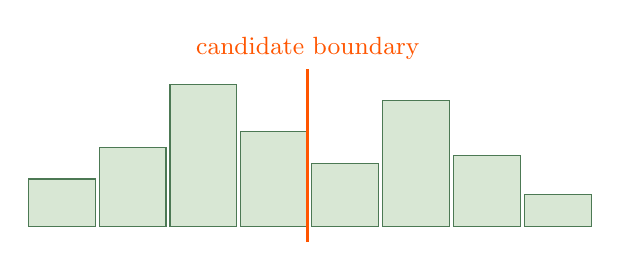
\begin{tikzpicture}
    \foreach \i/\hh in {0/.6,1/1.0,2/1.8,3/1.2,4/.8,5/1.6,6/.9,7/.4}{
      \draw[fill=bulletgreen!45,draw=forestgreen] (\i*.9,0) rectangle +(0.85,\hh);
    }
    \draw[slideorange,very thick] (3.55,-.2)--(3.55,2.0);
    \node[above,text=slideorange,font=\small] at (3.55,2.0) {candidate boundary};
  \end{tikzpicture}
  \vspace{.3cm}
  \par For missing values, compare adding their $G,H$ to the left or right child.
  \src{Schematic histogram.}
\end{frame}

\begin{frame}{OOB Coverage Across the Forest}
  For independent bootstrap samples across $B$ trees:
  \[q=\left(1-\frac1n\right)^m,\qquad
    K_i=|\mathcal B_i|\sim\operatorname{Binomial}(B,q).\]
  \[\E[K_i]=Bq,\qquad P(K_i=0)=(1-q)^B.\]
  \pause
  \vspace{.25cm}
  For large $n$, with $m=5n$ and $B=100$, each sample has about a $51\%$ probability of having no OOB tree.
  \vspace{.2cm}
  \begin{itemize}\spaceditems
    \item OOB error evaluates subensembles with varying numbers of trees.
    \item Repeated tuning against the OOB score can overfit the evaluation.
    \item Time dependence and grouped observations need suitable validation splits.
  \end{itemize}
\end{frame}

\begin{frame}{An Operational Case: Virtua Health, 2023}
  XGBoost ran hourly within the electronic medical record workflow at five hospitals.
  \vspace{.3cm}
  \centering
  \renewcommand{\arraystretch}{1.4}
  \begin{tabular}{lc}
    \toprule
    Reported operational metric & Value\\ \midrule
    XGBoost sensitivity & $91\%$\\
    XGBoost false-positive rate & $6\%$\\
    Existing commercial model's false-positive rate & $30\%$\\ \bottomrule
  \end{tabular}
  \vspace{.2cm}
  \par Three-week post-deployment evaluation: 1,896 patients, 98 sepsis cases.
  \vspace{.3cm}
  \par A matched-sensitivity comparison was not reported.\par
  Patient-outcome improvements were not established.
  \src{Optional discussion case.}
\end{frame}


\end{document}
